\documentclass[11pt, letterpaper]{article}
\usepackage[margin=1in]{geometry}
\usepackage{amsmath, amssymb}
\usepackage{graphicx}
\usepackage{booktabs}
\usepackage{float}
\usepackage{listings}
\usepackage{xcolor}
\usepackage[hidelinks]{hyperref}
\usepackage{caption}
\usepackage{parskip}

\definecolor{codebg}{RGB}{245,245,245}
\definecolor{codegreen}{RGB}{0,128,0}
\definecolor{codepurple}{RGB}{128,0,128}
\definecolor{codeblue}{RGB}{0,0,200}
\definecolor{coderule}{RGB}{180,180,180}
\definecolor{codenum}{RGB}{120,120,120}

\lstset{
  language=Python,
  backgroundcolor=\color{codebg},
  basicstyle=\ttfamily\small,
  keywordstyle=\color{codeblue}\bfseries,
  stringstyle=\color{codepurple},
  commentstyle=\color{codegreen}\itshape,
  numbers=left,
  numberstyle=\tiny\color{codenum},
  numbersep=8pt,
  frame=single,
  framerule=0.5pt,
  rulecolor=\color{coderule},
  breaklines=true,
  breakatwhitespace=true,
  showstringspaces=false,
  tabsize=4,
  captionpos=b,
}

\title{
  \textbf{ECE-GY 9143: High Performance Machine Learning}\\[6pt]
  \large Homework 4 --- Part B: Post-Training Quantization
}
\author{Haojing Tong \\ \texttt{[Your Student ID]}}
\date{Spring 2026}

\begin{document}
\maketitle
\tableofcontents
\newpage

%----------------------------------------------------------------------
\section{Introduction}
%----------------------------------------------------------------------

This report documents the implementation and analysis of post-training
quantization applied to a simple convolutional neural network (CNN) trained
on the CIFAR-10 dataset. Post-training quantization reduces the numerical
precision of a pre-trained model's weights, activations, and biases from
32-bit floating-point (\texttt{float32}) to low-precision fixed-point
integers: 8-bit signed integers (\texttt{int8}) for weights and activations,
and 32-bit signed integers (\texttt{int32}) for biases.

The key motivation is hardware efficiency: integer arithmetic requires
significantly less silicon area and memory bandwidth than floating-point
arithmetic, enabling deployment on resource-constrained ML accelerators.

\subsection{Model Architecture}

A six-layer CNN is trained on CIFAR-10 for two epochs using SGD
(lr$=0.001$, momentum$=0.9$). Baseline test accuracy: \textbf{52.70\%}.

\begin{itemize}
  \item \textbf{conv1}: Conv2d(3, 6, kernel=5, bias=False)
  \item \textbf{pool}: MaxPool2d(2, 2)
  \item \textbf{conv2}: Conv2d(6, 16, kernel=5, bias=False)
  \item \textbf{fc1}: Linear(400, 120, bias=False)
  \item \textbf{fc2}: Linear(120, 84, bias=False)
  \item \textbf{fc3}: Linear(84, 10, bias=False)
\end{itemize}

%----------------------------------------------------------------------
\section{Question 1: Visualize Weights}
%----------------------------------------------------------------------

\subsection{Method}

The weight tensor of each layer is flattened to a one-dimensional vector
and visualized as a histogram with 100 bins. The mean and $\pm3\sigma$
boundaries are overlaid to identify the effective dynamic range used for
subsequent quantization.

\subsection{Results}

\begin{figure}[H]
  \centering
  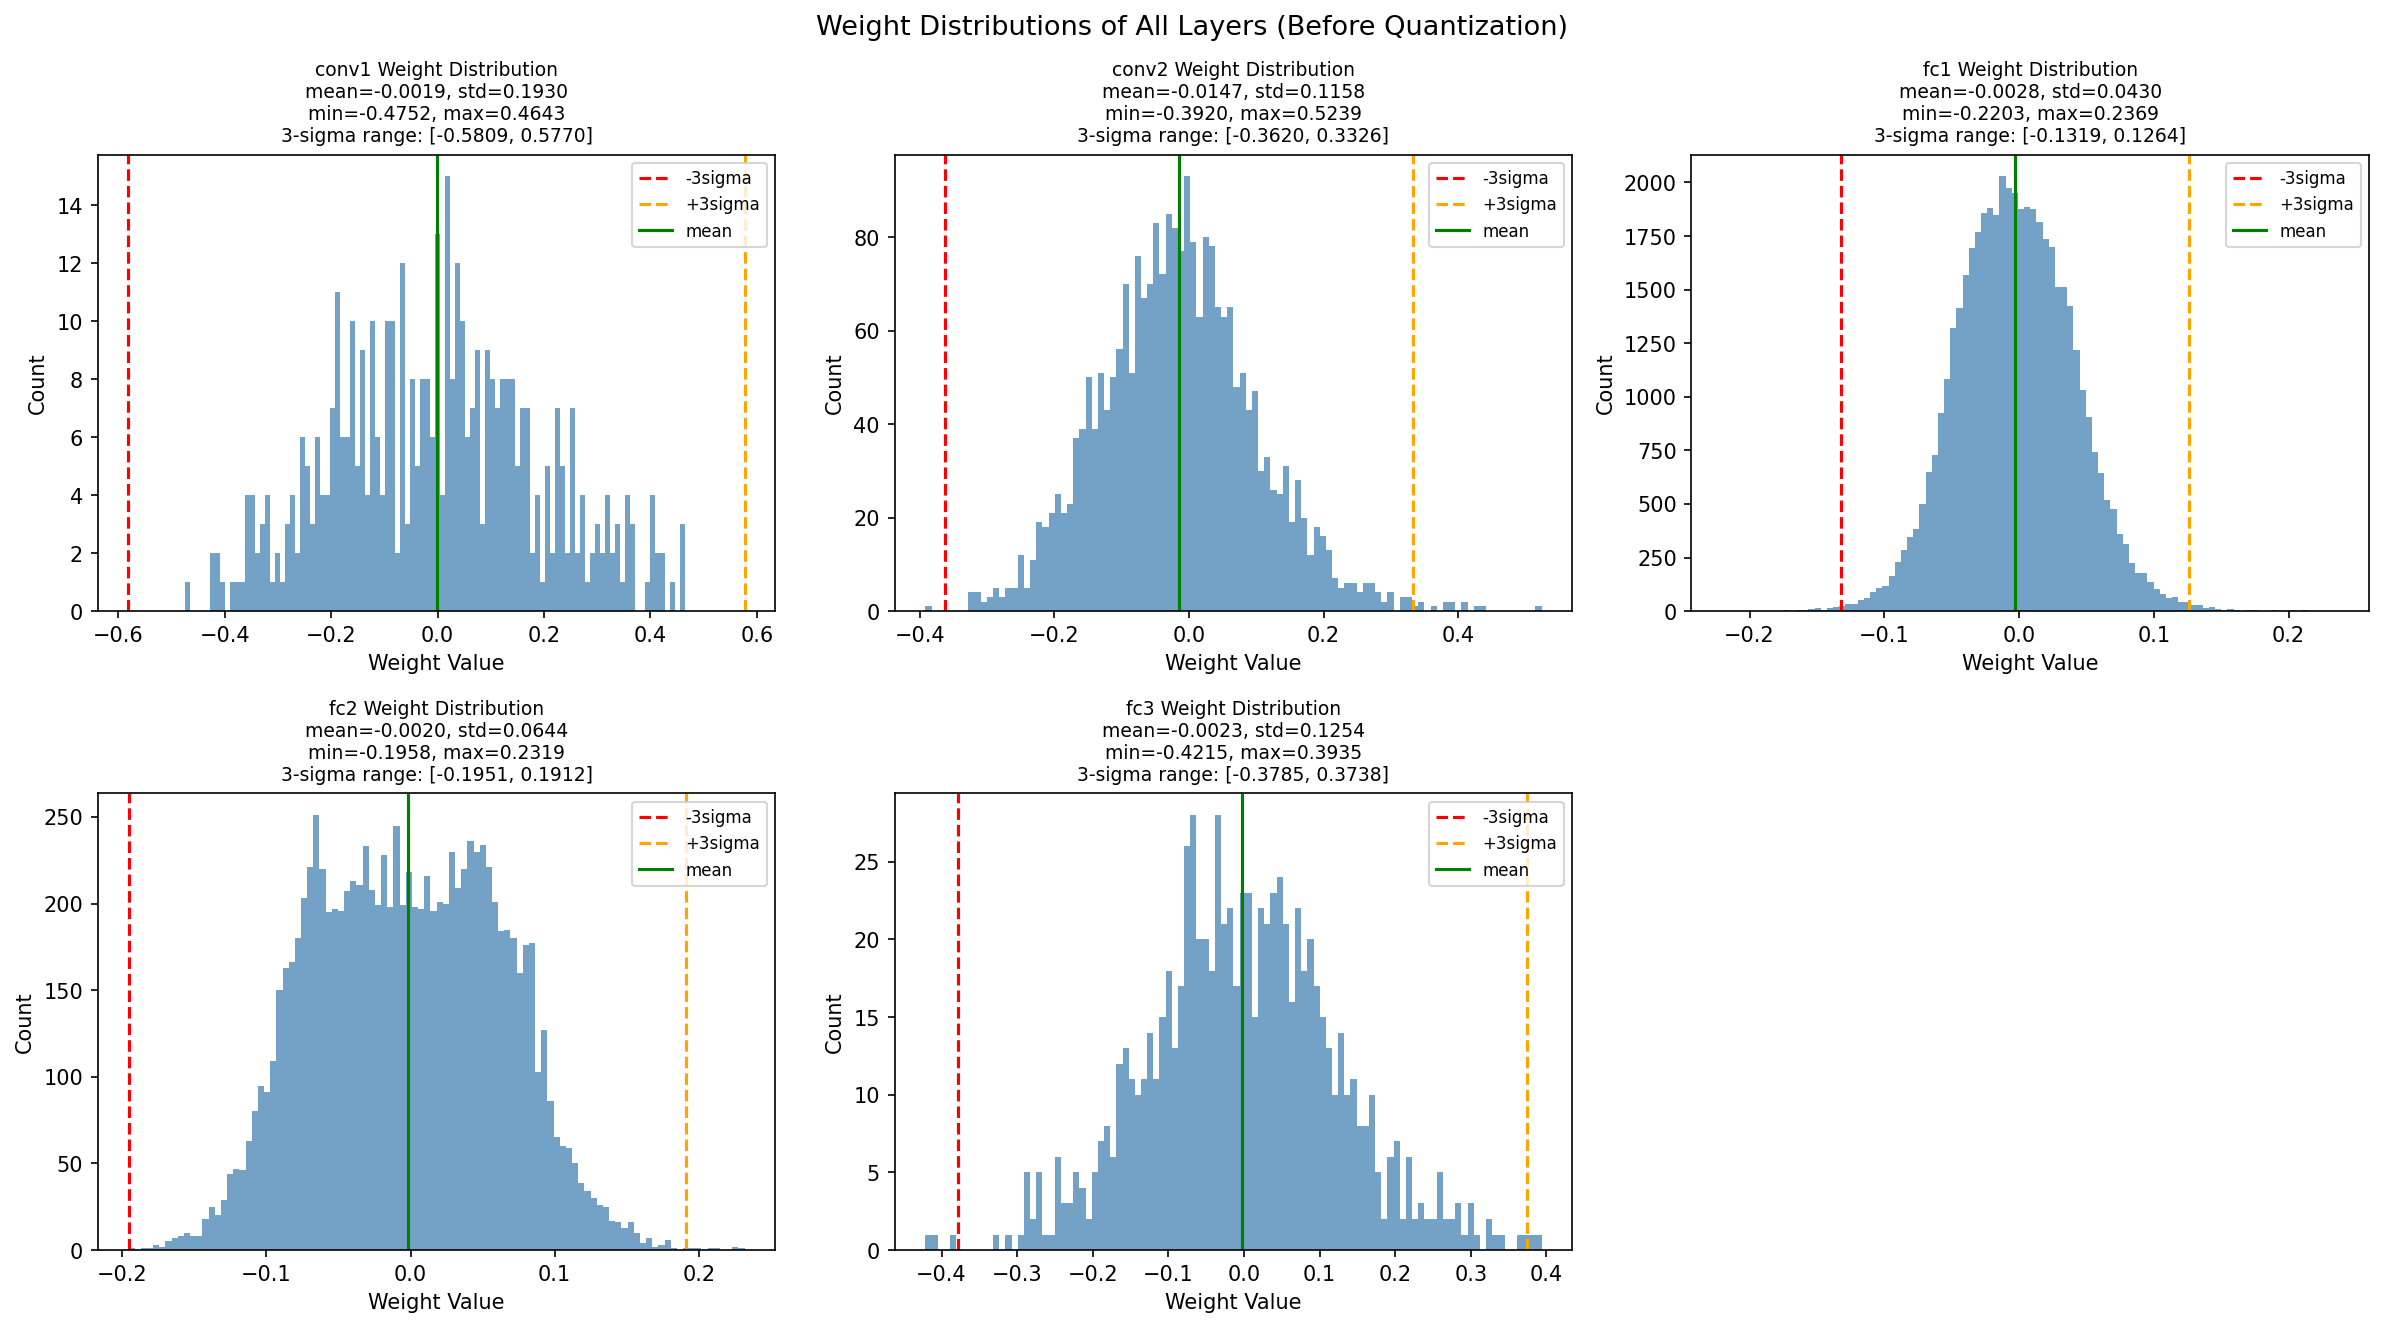
\includegraphics[width=\textwidth]{q1_weight_distributions.png}
  \caption{Weight distributions of all five layers before quantization.
           Green solid: mean. Red dashed: $-3\sigma$. Orange dashed: $+3\sigma$.}
  \label{fig:weights}
\end{figure}

\begin{table}[H]
  \centering
  \caption{Weight distribution statistics (before quantization).}
  \label{tab:weights}
  \begin{tabular}{lrrrrr}
    \toprule
    \textbf{Layer} & \textbf{Mean} & \textbf{Std}
                   & \textbf{Min}  & \textbf{Max}
                   & \textbf{$3\sigma$ range} \\
    \midrule
    conv1 & $-0.0019$ & $0.1930$ & $-0.4752$ & $0.4643$ & $[-0.581,\;0.577]$ \\
    conv2 & $-0.0147$ & $0.1158$ & $-0.3920$ & $0.5239$ & $[-0.362,\;0.333]$ \\
    fc1   & $+0.0028$ & $0.0430$ & $-0.2203$ & $0.2369$ & $[-0.132,\;0.126]$ \\
    fc2   & $-0.0020$ & $0.0644$ & $-0.1958$ & $0.2319$ & $[-0.195,\;0.191]$ \\
    fc3   & $-0.0023$ & $0.1254$ & $-0.4215$ & $0.3935$ & $[-0.379,\;0.374]$ \\
    \bottomrule
  \end{tabular}
\end{table}

\subsection{Observations}
\begin{itemize}
  \item All layers have weights centered tightly around zero (mean $\approx0$),
        consistent with well-behaved SGD training and symmetric weight initialization.
  \item The distributions are approximately Gaussian, which justifies the use of a
        $3\sigma$ clipping strategy for quantization.
  \item Fully-connected layers (fc1--fc3) have smaller standard deviations than
        convolutional layers (conv1, conv2), due to their larger parameter counts.
  \item The true min/max values are close to the $3\sigma$ boundary, meaning only
        a negligible fraction of weights would be clipped during quantization.
\end{itemize}

%----------------------------------------------------------------------
\section{Question 2: Quantize Weights}
%----------------------------------------------------------------------

\subsection{Quantization Strategy}

We use \textbf{symmetric $3\sigma$ scaling}. The scale factor $n_w$ is
chosen so that $\pm3\sigma$ of the weight distribution maps to $\pm127$:

\begin{equation}
  n_w = \frac{127}{3\,\sigma_w}.
  \label{eq:weight_scale}
\end{equation}

Each weight $w$ is then quantized by
$w_q = \mathrm{clamp}(\mathrm{round}(w \cdot n_w),\, -128,\, 127).$
Choosing $3\sigma$ rather than the absolute min/max makes the scale robust
to statistical outliers while keeping ${\approx}99.7\%$ of values within
the representable range.

\subsection{Code}

\begin{lstlisting}[caption={Weight quantization --- \texttt{quantized\_weights}.}]
def quantized_weights(weights):
    # Compute standard deviation of the weight distribution
    sigma = weights.std().item()
    # Scale so that +/-3*sigma maps to the full int8 positive range (127)
    scale = 127.0 / (3.0 * sigma)
    # Multiply, round to nearest integer, clamp to signed 8-bit range
    result = (weights * scale).round()
    result = torch.clamp(result, min=-128, max=127)
    return result, scale
\end{lstlisting}

\subsection{Results}

\begin{table}[H]
  \centering
  \caption{Accuracy before and after weight-only quantization.}
  \begin{tabular}{lc}
    \toprule
    \textbf{Model}                    & \textbf{Test Accuracy} \\
    \midrule
    Original (float32)                & 52.70\%                \\
    Weights quantized to int8         & \textbf{53.12\%}       \\
    \bottomrule
  \end{tabular}
\end{table}

Quantizing all weights to 8-bit integers yields a negligible accuracy change
($+0.42$ pp, within normal run-to-run variance). The slight increase suggests
that weight rounding acts as a mild regularizer for this small network,
confirming that the $3\sigma$ scaling strategy captures the meaningful weight
range without significant information loss.

%----------------------------------------------------------------------
\section{Question 3: Visualize Activations}
%----------------------------------------------------------------------

\subsection{Profiling Method}

PyTorch forward hooks are registered on every layer. During a profiling pass
over 400 training-set samples (no gradient computation), the hooks collect
the \emph{input} tensor to each layer---which equals the output of the
previous stage after any nonlinearity and pooling---as well as the final
logit output of fc3.

\subsection{Results}

\begin{figure}[H]
  \centering
  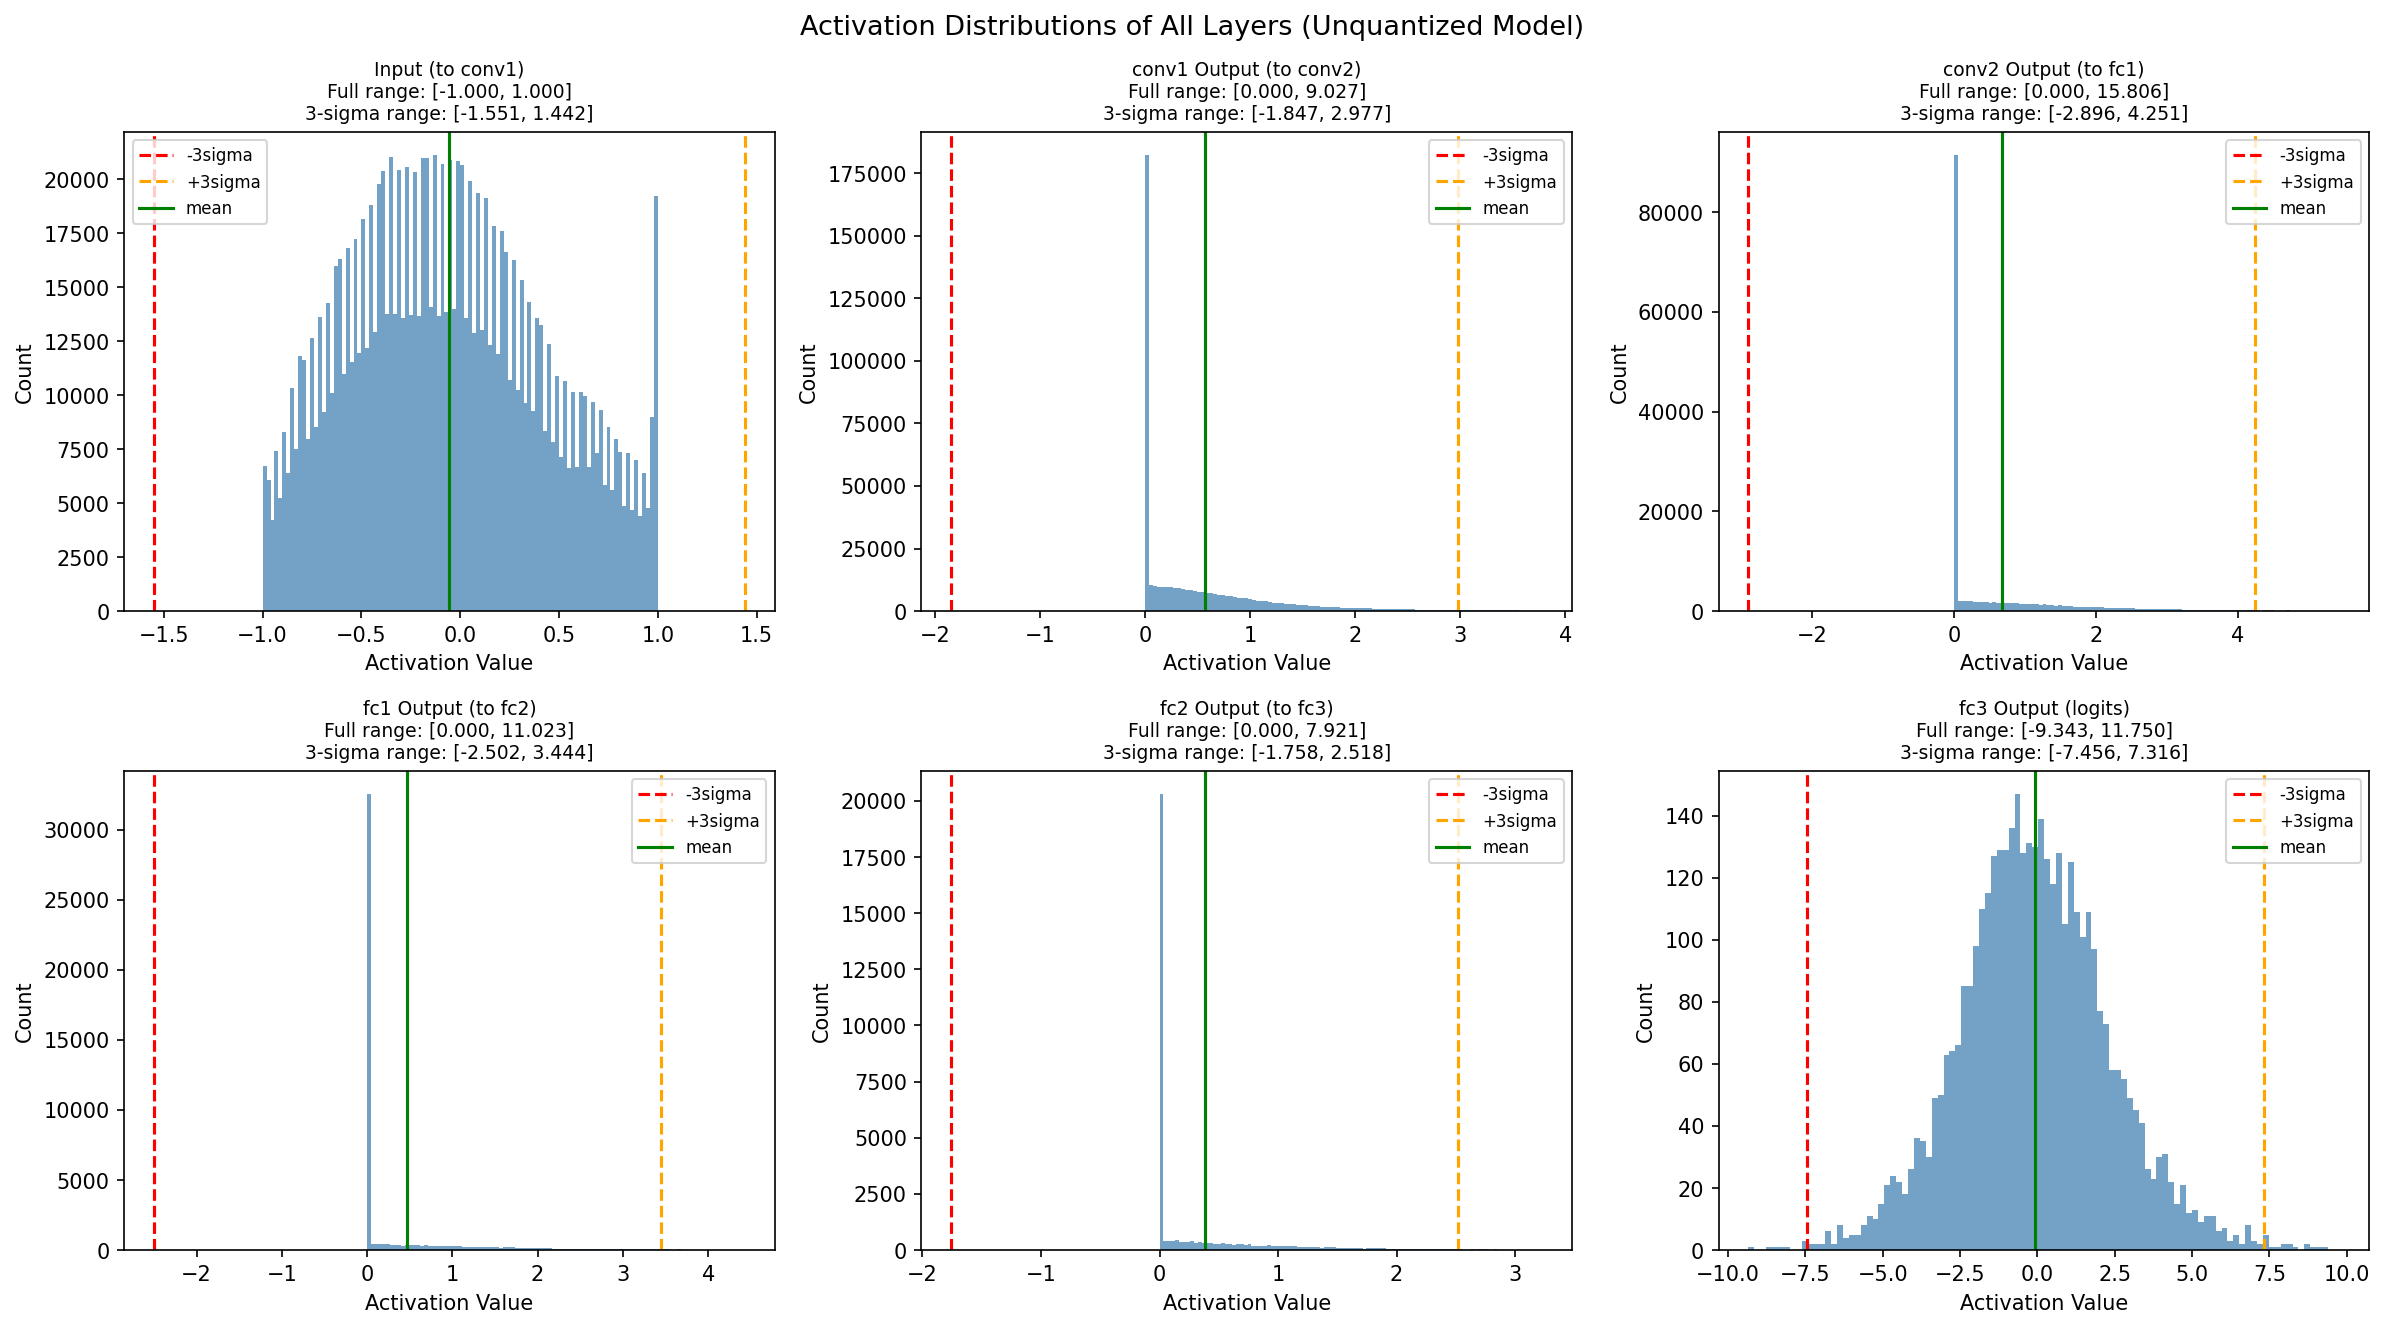
\includegraphics[width=\textwidth]{q3_activation_distributions.png}
  \caption{Activation distributions of all six stages (unquantized model).
           Green solid: mean. Red dashed: $-3\sigma$. Orange dashed: $+3\sigma$.}
  \label{fig:activations}
\end{figure}

\begin{table}[H]
  \centering
  \caption{Activation statistics across all layers.}
  \label{tab:activations}
  \begin{tabular}{lrrrrr}
    \toprule
    \textbf{Stage} & \textbf{Min} & \textbf{Max}
                   & \textbf{Mean} & \textbf{Std}
                   & \textbf{$3\sigma$ range} \\
    \midrule
    Input (to conv1)         & $-1.000$ & $1.000$  & $-0.055$ & $0.499$ & $[-1.551,\;1.442]$ \\
    conv1 output (to conv2)  & $0.000$  & $9.027$  & $0.565$  & $0.804$ & $[-1.847,\;2.977]$ \\
    conv2 output (to fc1)    & $0.000$  & $15.806$ & $0.677$  & $1.191$ & $[-2.896,\;4.251]$ \\
    fc1 output (to fc2)      & $0.000$  & $11.023$ & $0.471$  & $0.991$ & $[-2.502,\;3.444]$ \\
    fc2 output (to fc3)      & $0.000$  & $7.921$  & $0.380$  & $0.713$ & $[-1.758,\;2.518]$ \\
    fc3 output (logits)      & $-9.343$ & $11.750$ & $-0.070$ & $2.462$ & $[-7.456,\;7.316]$ \\
    \bottomrule
  \end{tabular}
\end{table}

\subsection{Observations}
\begin{itemize}
  \item \textbf{Input activations} follow a roughly uniform distribution in $[-1,1]$,
        as expected from CIFAR-10 normalization.
  \item \textbf{ReLU layers} (conv1--fc2 outputs) all have a hard lower bound of zero,
        producing heavily right-skewed distributions. The $3\sigma$ lower bound appears
        negative because $\sigma$ is computed from the skewed distribution; the effective
        quantization range in practice is $[0,\;\mu+3\sigma]$.
  \item \textbf{Activation magnitude grows} from conv1 (max $\approx9$) through conv2
        (max $\approx16$), reflecting the accumulation of many multiply-add operations
        across spatial positions in the convolutional layers.
  \item \textbf{Logit output} (fc3) is symmetric around zero with both positive and
        negative values, consistent with the absence of a final ReLU.
  \item The $3\sigma$ range captures the vast majority of activation values in all layers,
        confirming it is an appropriate clipping boundary for quantization.
\end{itemize}

%----------------------------------------------------------------------
\section{Question 4: Quantize Activations}
%----------------------------------------------------------------------

\subsection{Theoretical Background}

In integer inference every value is represented as a scaled integer.
Let $n_0$ be the input scale, $n_{w,l}$ the weight scale of layer $l$,
and $s_l$ its output scale. The \emph{accumulated scale} before layer $l$'s
output rescaling is

\begin{equation}
  A_l = n_0 \cdot n_{w,l} \cdot \prod_{i=1}^{l-1} n_{w,i}\cdot s_i.
  \label{eq:acc_scale}
\end{equation}

The output scale is chosen so that $3\sigma$ of the float activations maps to 127:

\begin{equation}
  s_l = \frac{127}{3\,\sigma_{\mathrm{act},l} \cdot A_l}.
  \label{eq:output_scale}
\end{equation}

\subsection{Code}

\begin{lstlisting}[caption={Scale for the initial input --- \texttt{quantize\_initial\_input}.}]
@staticmethod
def quantize_initial_input(pixels):
    # 3-sigma strategy: +/-3*sigma maps to +/-127
    sigma = np.std(pixels)
    scale = 127.0 / (3.0 * sigma)   # e.g. 127/(3*0.499) ~ 84.8
    return scale
\end{lstlisting}

\begin{lstlisting}[caption={Per-layer output scale --- \texttt{quantize\_activations}.}]
@staticmethod
def quantize_activations(activations, n_w, n_initial_input, ns):
    # Build accumulated scale A_l = n_0 * n_w * product of preceding (n_w_i * s_i)
    accumulated_scale = n_initial_input * n_w
    for (n_w_prev, n_out_prev) in ns:
        accumulated_scale *= n_w_prev * n_out_prev
    sigma = np.std(activations)
    if sigma == 0:
        return 1.0    # all activations are zero (fully clipped by ReLU)
    output_scale = 127.0 / (3.0 * sigma * accumulated_scale)
    return output_scale
\end{lstlisting}

\begin{lstlisting}[caption={Quantized forward pass --- \texttt{NetQuantized.forward}.}]
def forward(self, x):
    # Quantize float input to int8
    x = (x * self.input_scale).round().clamp(-128, 127)
    # conv1: int MAC -> ReLU -> MaxPool -> rescale to int8
    x = self.conv1(x)
    x = F.relu(x)
    x = self.pool(x)
    x = (x * self.conv1.output_scale).round().clamp(-128, 127)
    # conv2: int MAC -> ReLU -> MaxPool -> rescale to int8
    x = self.conv2(x)
    x = F.relu(x)
    x = self.pool(x)
    x = (x * self.conv2.output_scale).round().clamp(-128, 127)
    # Flatten spatial feature map
    x = x.view(-1, 16 * 5 * 5)
    # fc1: int MAC -> ReLU -> rescale to int8
    x = self.fc1(x)
    x = F.relu(x)
    x = (x * self.fc1.output_scale).round().clamp(-128, 127)
    # fc2: int MAC -> ReLU -> rescale to int8
    x = self.fc2(x)
    x = F.relu(x)
    x = (x * self.fc2.output_scale).round().clamp(-128, 127)
    # fc3: final logits -- no re-quantization needed
    x = self.fc3(x)
    return x
\end{lstlisting}

\subsection{Results}

\begin{table}[H]
  \centering
  \caption{Accuracy at each quantization stage.}
  \begin{tabular}{lcc}
    \toprule
    \textbf{Model}                           & \textbf{Test Acc.} & \textbf{$\Delta$} \\
    \midrule
    Original (float32)                       & 52.70\%   & ---         \\
    Weights quantized (int8)                 & 53.12\%   & $+0.42$ pp  \\
    Weights + activations quantized (int8)   & \textbf{52.84\%}  & $-0.14$ pp  \\
    \bottomrule
  \end{tabular}
\end{table}

Quantizing both weights and activations to int8 yields \textbf{52.84\%} accuracy,
a degradation of only $0.14$ pp relative to float32. This near-zero accuracy loss
validates the correctness of the cumulative scale tracking in
Equations~\eqref{eq:acc_scale}--\eqref{eq:output_scale}.

%----------------------------------------------------------------------
\section{Question 5: Quantize Biases}
%----------------------------------------------------------------------

\subsection{Theoretical Background}

In integer hardware a layer's computation is
$Y = W^{(q)} \cdot X^{(q)} + b^{(q)}.$
The dot product $W^{(q)}\cdot X^{(q)}$ accumulates into a \textbf{32-bit integer}
register. The bias must be on exactly the same scale as this accumulator:

\begin{equation}
  b^{(q)} = \mathrm{clamp}\\!\left(
    \mathrm{round}(b_{\mathrm{float}} \cdot A_l),\;
    -2^{31},\; 2^{31}-1
  \right),
  \label{eq:bias_quant}
\end{equation}

where $A_l$ is the same accumulated scale from Equation~\eqref{eq:acc_scale}.
Biases use \texttt{int32} (not \texttt{int8}) because the accumulator is 32-bit,
providing sufficient range to avoid overflow.

\subsection{Code}

\begin{lstlisting}[caption={Bias quantization to int32 --- \texttt{quantized\_bias}.}]
@staticmethod
def quantized_bias(bias, n_w, n_initial_input, ns):
    # Build the same accumulated scale as the weight-input dot product
    accumulated_scale = n_initial_input * n_w
    for (n_w_prev, n_out_prev) in ns:
        accumulated_scale *= n_w_prev * n_out_prev
    # Scale the float bias, round to nearest integer, clamp to int32 range
    bias_q = (bias * accumulated_scale).round()
    return torch.clamp(bias_q, min=-2147483648, max=2147483647)
\end{lstlisting}

\subsection{Results}

\begin{table}[H]
  \centering
  \caption{Accuracy for the bias-enabled network at each quantization stage.}
  \label{tab:bias}
  \begin{tabular}{lcc}
    \toprule
    \textbf{Model}                                       & \textbf{Test Acc.} & \textbf{$\Delta$} \\
    \midrule
    Net with bias (float32)                              & 51.24\%   & ---         \\
    Weights int8, bias \textbf{not} quantized (float)   & 46.56\%   & $-4.68$ pp  \\
    Weights int8 + bias \textbf{int32} (aligned)        & \textbf{49.54\%}  & $-1.70$ pp  \\
    \bottomrule
  \end{tabular}
\end{table}

\subsection{Analysis}

\paragraph{Weights int8, bias float32 (46.56\%).}
When weights are scaled by $n_w$ (turning them into integers $\sim100$) but the
bias remains a small float ($\sim0.01$--$1.0$), the two operands differ by many
orders of magnitude. Adding a float bias to an int32 accumulator that has been
amplified by $A_l$ is numerically equivalent to adding nearly zero---the bias
contribution is effectively lost, causing a $4.68$ pp accuracy drop.

\paragraph{Weights int8 + bias int32 (49.54\%).}
Quantizing the bias with the same accumulated scale $A_l$ ensures it occupies
the correct magnitude inside the 32-bit accumulator. Accuracy recovers by
$\approx3$ pp. The remaining $1.70$ pp gap reflects the irreducible quantization
noise of full int8 inference.

This experiment conclusively demonstrates that \textbf{all parameters added to
an integer accumulator must share the same integer scale}, and that using 32-bit
integers for biases provides sufficient precision to avoid overflow.

%----------------------------------------------------------------------
\section{Conclusion}
%----------------------------------------------------------------------

\begin{table}[H]
  \centering
  \caption{Accuracy summary across all quantization stages.}
  \label{tab:summary}
  \begin{tabular}{lcc}
    \toprule
    \textbf{Quantization Stage}                    & \textbf{Accuracy} & \textbf{$\Delta$ vs.\ float} \\
    \midrule
    Float32 baseline                               & 52.70\%  & ---         \\
    Weights int8                                   & 53.12\%  & $+0.42$ pp  \\
    Weights int8 + Activations int8                & 52.84\%  & $-0.14$ pp  \\
    \midrule
    Float32 baseline (with bias)                   & 51.24\%  & ---         \\
    Weights int8, bias float (scale mismatch)      & 46.56\%  & $-4.68$ pp  \\
    Weights int8 + bias int32 (aligned)            & 49.54\%  & $-1.70$ pp  \\
    \bottomrule
  \end{tabular}
\end{table}

The key conclusions are:
\begin{enumerate}
  \item \textbf{$3\sigma$ scaling} is an effective heuristic for quantization:
        robust to outliers while preserving nearly all dynamic range.
  \item \textbf{Weight-only quantization} introduces negligible accuracy loss,
        showing that int8 weights nearly losslessly compress float32 weights.
  \item \textbf{Activation quantization} with properly tracked cumulative scales
        also preserves accuracy ($-0.14$ pp), validating the scale propagation theory.
  \item \textbf{Bias quantization} must use the same accumulated scale as the
        weight--input dot product. A scale mismatch causes a $4.68$ pp drop;
        properly aligned int32 bias quantization limits the drop to $1.70$ pp.
\end{enumerate}

\end{document}